% !TEX root = ../agglo_clust_review.tex

\section{Generalized framework for Signed Graphs Agglomerative Clustering}
In this section we introduce the proposed framework for agglomerative clustering of signed graphs. 
%that represents a simple \UPDATE{generalized} formalization of many agglomerative graph clustering algorithms. \UPDATE{It can be used to describe both unsigned clustering algorithms ingesting positive node similarities and signed clustering algorithms using attractive and repulsive cues.}\\
First, we define the graph notation in Sec. \ref{sec:notation}, then we introduce the generalized algorithm in Sec. \ref{sec:algorithm} and finally we show \UPDATE{how it can be seen as a generalization of existing and new graph clustering algorithms in Sec. \ref{sec:alg_update_rules}.}

\subsection{Notation and graph formalism} \label{sec:notation}

We consider an undirected simple graph $\mathcal{G}(V,E)$, in which nodes can represent either pixels, superpixels or voxels. We call the set $\Pi$ a \emph{clustering} with $K$ clusters if $V = \cup_{i=1}^K S_i $, $S_i \cap S_j = \emptyset$ for each $i\neq j$ and every $S \in \Pi$ induces a connected subgraph of $\mathcal{G}$. In the following we denote as $S_u$ the cluster associated with node $u$.
% \begin{equation}
% S_u \equiv S \in \Pi \,\, \text{s.t.} \,\, u \in S
% \end{equation}

In this work, we consider the problem of clustering a weighted graph $\mathcal{G}(V,E,w^+, w^-)$ with both attractive and repulsive edge attributes. The weight function $w^+: E \rightarrow \mathbb{R}^+$ associates a positive scalar attribute $w_e^+\in \mathbb{R}^+$ representing a merge affinity or a similarity measure: the higher this number, the higher the inclination of the two incident vertices to be assigned to the same cluster\footnote{Note that several formalisms for positively weighted graphs associate to each edge a positive scalar that represents a metric or distance on the graph, thus, the \emph{lower} the edge weight, the higher the attraction between the two linked nodes, contrary to our definition of $w^+: E \rightarrow \mathbb{R}^+$.}. On the other hand, $w^-: E \rightarrow \mathbb{R}^+$ associates a split tendency $w_e^- \in \mathbb{R}^+$: the higher this weight, the more the incident vertices would like to be in different clusters. 
Graphs of the type $\mathcal{G}(V,E,w^+, w^-)$ are also often defined as \emph{signed graphs} $\mathcal{G}(V,E,\cost)$, featuring signed edge weights: ${\cost_e = w_e^+ - w_e^- \in \mathbb{R}, \, \forall e \in E}$.
Graphs with purely attractive interactions are a special case of $\mathcal{G}(V,E,\cost)$ with $\cost_e \geq 0$ and $w^-_e=0$ for each $e \in E$.

\paragraph{Inter-cluster interaction}\label{par:linkage_criterion_def} We call two clusters $S_1,S_2$ \emph{adjacent} if there exists at least one edge ${e_{uv}\in E}$ connecting a node $u\in S_1$ to a node $v\in S_2$. In agglomerative HC, the interaction $\interact_{S_1,S_2}$ between two clusters $S_1, S_2$ is usually defined as a function, named \emph{linkage criterion}, depending on the weights of all edges connecting clusters $S_1$ and $S_2$. For example, for a \emph{maximum} linkage criterion statistic (single-linkage), the inter-cluster interaction is given by:
\begin{equation}\label{eq:max_linkage}
\interact_{S_1,S_2} = \, \max_{e\in U(S_u,S_v)} \cost(e), \qquad \text{where}\quad E_{12} = \{ e_{uv} \in E | u \in S_1, \, v \in S_2 \}.
\end{equation}
Other common choices are \emph{minimum} (complete linkage) or \emph{average} (average linkage). %and \emph{sum}.
% \begin{equation}
%  \text{$S_1, S_2 \in \Pi$ are \emph{adjacent}} \quad \Longleftrightarrow  \quad  \mathcal{B}(S_1,S_2) \equiv \{ e_{uv} \in E | u \in S_1, \, v \in S_2 \} \neq \emptyset
% \end{equation}
% where we defined the set of edges connecting two adjacent clusters as \UPDATE{\emph{boundary}} \UPDATE{$\mathscr{W}(S_1,S_2) , \mathcal{G}'_{\mathcal{G},\Pi}(V',E')$}.  in the boundary $\mathcal{B}(S_1,S_2)$. Some examples of linkage criterion statistics are \emph{maximum} (single-linkage), \emph{minimum} (complete-linkage) and average (average-linkage).

\paragraph{Multicut and correlation clustering} For any clustering $\Pi$ of $\mathcal{G}$, we define as $E^0_\Pi$ the set of edges linking nodes in the same cluster, and as $E_\Pi^1$ the complementary set of edges whose linked nodes belong to distinct clusters:
\begin{equation}
E_\Pi^0 \equiv \{ e_{uv} \in E \,|\, \exists S \in \Pi : u \in S \, \text{and} \, v \in S \}, \qquad E^1_\Pi \equiv E \setminus E^0_\Pi.
\end{equation}
% \begin{align}
% E_\Pi^0 &= \{ e_{uv} \in E \,|\, \exists S \in \Pi : u \in S \, \text{and} \, v \in S \}, \\
% E^1_\Pi &= E \setminus E^0_\Pi.
% \end{align}
The set of edges $E_\Pi^1$ is known as the \emph{multicut} of $\mathcal{G}$ w.r.t. clustering $\Pi$. The instance of the NP-hard \emph{weighted correlation clustering} or \emph{minimum cost multicut problem} w.r.t. $\mathcal{G}(V,E,w^+, w^-)$ \cite{kappes2011globally,chopra1991multiway,andres2015lifting} is the task of finding the clustering that optimally balance the attraction and repulsion in the graph and is given by the following optimization problem/binary integer program:
\begin{equation}
% \min_\Pi \texttt{MC}(\Pi) \equiv
 \min_\Pi \sum_{e\in E} \cost_e x_e^\Pi,  \qquad \text{where} \quad x^\Pi_e = 
 \begin{cases} 
 1 & \text{if } e\in E^1_\Pi \\
 0 & \text{otherwise}.
 \end{cases}
\end{equation}
In the next chapters we will use this objective as a way to measure how much a clustering is balanced.

\begin{figure}
\centering
        \begin{subfigure}[t]{0.46 \textwidth}
        \centering
        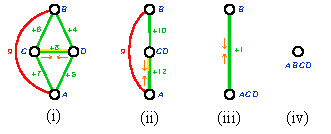
\includegraphics[width=\textwidth]{./figs/example_no_constr.pdf}
        \caption{No constraints}
    \end{subfigure} \hfill
    \begin{subfigure}[t]{0.46 \textwidth}
        \centering
        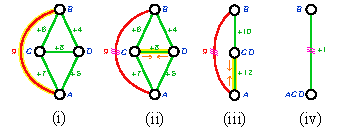
\includegraphics[width=\textwidth]{./figs/example_with_constr.pdf}
        \caption{With constraints}
    \end{subfigure}
\caption{Some iterations of the generalized algorithm with and without adding cannot-link constraints. In this example the \emph{Sum} linkage criteria was used. The graph has both attractive (green) and repulsive (red) edges and cannot-link constraints are shown with triple violet bars on the edges. We note that when constraints are enforced, the final clustering is given by two clusters instead of only one.}
\label{fig:algorithm_with_without_CLC}
\end{figure}
\begin{algorithm}[t]
  \caption{Generalized Algorithm for Signed Graphs Agglomerative Clustering}
   \hspace*{\algorithmicindent} \textbf{Inputs:} Graph $\mathcal{G}(V,E,w^+,w^-)$ with $N$ nodes; boolean variable {\color{blue}\texttt{addCannotLink}}  \\
  \hspace*{\algorithmicindent} \textbf{Outputs:} Final clustering $\Pi$\\
  \hspace*{\algorithmicindent} 
  \begin{algorithmic}[1]
    % \Procedure{SignedGraphEdgeContr}{{\color{blue}bool \emph{addConstraints}}}
      % \State $\mathcal{G}'\gets \mathcal{G}(V,E^+ \cup E^-)$ \Comment{Initialize the contracted graph}
      \State Initialize clustering $\Pi=\{\{v_1\}, \ldots, \{v_N\}\}$ and contracted graph $\tilde{\mathcal{G}}_\Pi \gets \mathcal{G}$
      \State Initialize \texttt{canBeMerged}$[e] \gets$ \texttt{True} $\,\,\, \forall e\in E$
      \State Sort edges in priority queue (PQ) in descending order of priority $|\cost_e|=|w^+_e - w^-_e|$ 
      \State
      \While{PQ is \textbf{not} empty}
        \State Pop edge $e_{uv}$ in $\tilde{\mathcal{G}}_\Pi$ with highest absolute interaction $|\tilde{\cost}|$
        \If{({\color{ForestGreen}\textbf{$\tilde{\cost} > 0$}}) \textbf{and} \texttt{canBeMerged}$[e_{uv}]$}
          % \State PQ, $\,E_\dagger,\,\, E' \gets$ \textsc{deleteDoubleEdges}($u,v$)
        %   \State Update costs of double edges;
        %   \State Propagate constrained flags of double edges;
          \State Contract $e_{uv}$ in $\tilde{\mathcal{G}}_\Pi$ and merge the two clusters $S_u,S_v \in \Pi$
          \For{every new pair of double edges $(e_1,e_2)$ in $\tilde{\mathcal{G}}_\Pi$}
            % \State Get costs $\cost_1, \cost_2$ of $e_1,e_2$
            \State Delete $e_2$ from $\tilde{\mathcal{G}}_\Pi$ and update priority of $e_1$ with rule $f(\tilde{\cost}_{e_1},\tilde{\cost}_{e_2})$ defined in Tab. \ref{tab:linkage-criteria} 
            % \Statex \hspace{\algorithmicindent}\hspace{\algorithmicindent}\hspace{\algorithmicindent}\hspace{\algorithmicindent} update priority of $e_1$
            % \State Delete $e_2$ from $\mathcal{G}'$
          \EndFor
          % \State  Replace double edges in $\mathcal{G}'$ with single edges
          % \Statex \hspace{\algorithmicindent}\hspace{\algorithmicindent}\hspace{\algorithmicindent} and update priorities
        \EndIf
        % \State
        \If{({\color{red}\textbf{$\tilde{\cost} \leq 0$}}) \textbf{and} {\color{blue}\texttt{addCannotLink}}}
          % \State Flag $e_{uv}$ as MustNotLink
          \State \texttt{canBeMerged}$[e_{uv}] \gets$ \texttt{False}
        \EndIf
      \EndWhile
      % \For{$e  \in E$ in descending order of absolute costs $|W(e)|$}
      %   \If{({\color{ForestGreen}\textbf{$W(e) > 0$}}) \textbf{AND} (edge is not constrained)}
      %     \State Contract edge $e$ in the graph $\mathcal{G}'$;
      %     \State Update costs of double edges;
      %     \State Propagate constrained flags of double edges;
      %     % \For{every new double edge}
      %     %   \State Delete double edges
      %     %   \State Insert new one with updated cost
      %     % \EndFor
      %   \EndIf
      %   \If{({\color{red}\textbf{$W(e) \leq 0$}}) \textbf{AND} ({\color{blue}\emph{addConstraints}})}
      %     \State Flag edge $e$ as constrained
      %   \EndIf
      % \EndFor
      % \State
      \State
      \Return $\Pi$
      % \State
    % \EndProcedure
  \end{algorithmic}
  \label{main_alg}
\end{algorithm}



\subsection{Generalized Algorithm for Signed Graphs Agglomerative Clustering} \label{sec:algorithm}

We now present a Generalized Algorithm for Signed Graphs Agglomerative Clustering (\algname) that describes several graph partitioning algorithms previously introduced in the literature and highlights the existence of new ones.

The proposed algorithm \ref{main_alg} uses a bottom-up approach starting with each node assigned to its own cluster and iteratively merges pairs of adjacent clusters. Intuitively, the algorithm starts by merging clusters with the strongest attractive interaction, corresponding to the highest positive weights in the graph, and it stops when the remaining clusters share only mutual repulsive interactions (see Fig. \hyperref[fig:intro_figure]{\ref*{fig:intro_figure}b} and \hyperref[fig:intro_figure]{\ref*{fig:intro_figure}c}). 

A second variant of the proposed algorithm also introduces \emph{cannot-link constraints}, representing mutual exclusion relationships between pairs of nodes that cannot be associated with the same cluster in the final clustering. This variant (Algorithm \ref{main_alg} with \texttt{addCannotLink=True}) stops when all the remaining clusters have been previously constrained.
% The algorithm that we will present in the next section iteratively performs a sequence of so-called \emph{edge contractions} on the original graph $\mathcal{G}(V,E,w^+, w^-)$.
% The graph clustering algorithm we will present in Sec. \ref{sec:algorithm} is a bottom-up approach starting with each node assigned to its own cluster and iteratively merging clusters. During the agglomeration, the current clustering $\Pi$ is represented by a \emph{contracted graph} $\mathcal{G'}(\mathcal{G}, \Pi)$, such that each of its nodes represents a cluster $S \in \Pi$ and \emph{adjacent} clusters are linked by an edge. 

\paragraph{Update rules} During the agglomerative process, the interaction between adjacent clusters has to be properly updated and recomputed.  % given by the linkage criterion defined in Sec. \ref{sec:notation} and
An efficient way of implementing these updates can be achieved by representing the agglomeration as a sequence of \emph{edge contractions} in the graph. Given a graph $\mathcal{G}(V,E,\cost)$ and a clustering $\Pi$, we define the associated \emph{contracted graph} $\tilde{\mathcal{G}}_\Pi(\tilde{V}, \tilde{E}, \tilde{\cost})$, such that $\tilde{V} \subseteq V$ and each node $u\in \tilde{V}$ represents the cluster $S_u \in \Pi$ including $u\in V$. Edges in $\tilde{E}$ represent adjacency-relationships between clusters and the signed edge weights $\tilde{\cost}_e$ are given by inter-cluster interactions $\tilde{\cost}(e_{uv})=\interact_{S_u,S_v}$. 
For the linkage criteria tested in this work, when two clusters $S_u$ and $S_v$ are merged, the interactions between the new cluster $S_u \cup S_v$ and each of its neighbors depend only on the previous interactions involving $S_u$ and $S_v$. Thus, we can easily recompute these interactions by using a simple \emph{update rule} $f$ that does not involve any loop over the edges of the original graph $\mathcal{G}$. As an example, given the single-linkage criterion defined in Eq. \ref{eq:max_linkage}, the interaction between $S_u \cup S_v$ and one of its neighbors $S_t$ is simply given by:
\begin{equation}
  \interact_{S_u \cup S_v,S_t} = f( \interact_{S_u,S_t}, \interact_{S_v,S_t}) = f(\tilde{\cost}(e_{ut}), \tilde{\cost}(e_{vt})) = \max \{ \tilde{\cost}(e_{ut}), \tilde{\cost}(e_{vt}) \}
\end{equation}
All the update rules tested in this article are listed in Table \ref{tab:linkage-criteria}.
% \UPDATE{Every time a pair of clusters is merged, the contracted graph is updated by performing an edge contraction and merging the associated nodes. The only interactions that then need to be updated are those between nodes that after the edge contraction happen to be connected by double edges (see Fig. \ref{fig:edge_contraction_and_contr_graph}, step b). For basic linkage criteria, e.g. \emph{max} or \emph{min}, the new interaction can be formulated in terms of an \emph{update rule} $f$ depending only on the these updates can be computed with an update rule $f$ that depends only on the interactions at the previous step }
% As a result, the merged node could be linked to some of its neighbors by double edges . , representing the fact that their interaction should be updated. This update can be easily achieved by using an \emph{update rule} depending only on the weights of the double edges. 
% \TODO{such a mess...} ...without the need of running a loop over the edges of the original graph.
% \UPDATE{In this way we do not need to recompute the interaction by using the linkage criterion over all the edges of the original graph, that would be computationally expensive.}
\paragraph{The proposed edge contraction algorithm} Algorithm \ref{main_alg} then proceeds as follows, similarly to the one presented in \cite{levinkov2017comparative}. It starts with each node assigned to its own cluster and sorts all edges $e\in E$ in a priority queue (PQ) by their absolute weight $|\cost_e|=|w_e^+ - w_e^-|$ in descending order, so that the most attractive and the most repulsive interactions are processed first. It then iteratively pops one edge $e_{uv}$ from PQ and, depending on the priority $\tilde{\cost}$, does the following: in case of attractive interaction $\tilde{\cost}>0$, provided that $e_{uv}$ was not flagged as a cannot-link constraint, then merge the connected clusters, perform an edge contraction of $e_{uv}$ in $\tilde{\mathcal{G}}_\Pi$ and update the priorities of new double edges as explained in Fig. \ref{fig:edge_contraction_and_contr_graph}. 
% For every new pair of double edges in $\tilde{\mathcal{G}}_\Pi$, update their priorities according to one of the update rules listed in Table \ref{tab:linkage-criteria} together with their cannot-link relationships. 
If, on the other hand, the interaction is repulsive ($\tilde{\cost}\leq 0$) and the option \texttt{addCannotLink} of Alg. \ref{main_alg} is \texttt{True}, then the edge $e_{uv}$ is flagged as cannot-link constraint.
In the Supplementary material we comment on the algorithm computational complexity (Sec. \ref{sec:complexity}).

 %\TODO{use def of merging process of contracted graph to define merging tree?}.

% \item Comment about must-not-link relations: they give high priority to the most confident repulsive edges {}


% Given a clustering $\Pi$ and a graph $\mathcal{G}(V,E,W)$, the interaction between two clusters $S_1, S_2 \in \Pi$ is usually defined in terms of a \emph{linkage criterion}, i.e. a function of all the edge weights connecting the two clusters:
% \begin{equation} 
% \begin{gathered}
% \mathcal{L}(S_1,S_2) = \mathcal{L}(\mathcal{W})\quad \\
%    \text{where} \quad \mathcal{W} = \{ W(e_{uv})| u\in S_1, v\in S_2 \}.
% \end{gathered}
% \end{equation}


\begin{table*}
    \centering
    \scriptsize
    \begin{subtable}[t!]{\textwidth}\centering
        \begin{tabular}{c r  l ?? c | c | c}
            % \toprule\toprule
            \multicolumn{3}{c??}{}  & \multirow{2}{*}[-0.5em]{\textbf{Unsigned Graphs}} & \multicolumn{2}{c}{\textbf{Signed Graphs}}  \\        
            % \cmidrule(l{.15em}){4-5}
            % \cline{4-5}
            % \multicolumn{2}{c||}{} &  &  \multicolumn{2}{c}{\thead{Add Cannot-Link Constraints:}} \\        
            \multicolumn{3}{c??}{} &  &  \multicolumn{1}{c}{\thead{No Constraints}} & \thead{With Constraints} \\        
      
            % \midrule[0.15em]
            \cmidrule[0.15em]{2-6}\morecmidrules \cmidrule[0.15em]{2-6}
            % \midrule \midrule
            \multirow{5}{*}[-2.5em]{\begin{turn}{90}\thead{\textbf{Linkage criteria} $\,\,\interact_{S_u ,S_v}$}\end{turn}}  & Sum: & $\displaystyle \sum_{e\in (S_u \times S_v)} \cost_e$ & \thead{Sum Linkage\\Hier. Aggl. Clust.} & \thead{Greedy Additive \\ Edge Contraction \cite{keuper2015efficient}} & \thead{Greedy Fixation\\\cite{levinkov2017comparative}} \\ 
            \cmidrule[0.07em]{2-6}
            
             &\makecell[r]{Absolute \\Max:} & 
            $\displaystyle \cost_e$ with $\displaystyle e = \argmax_{t\in (S_u \times S_v)} |\cost_t|$
               & \thead{Single Linkage\\Hier. Aggl. Clust. \cite{lance1967general}} & \thead{Mutex Watershed \\\cite{wolf2018mutex}} & \thead{Mutex Watershed\\\cite{wolf2018mutex}} \\
              \cmidrule[0.07em]{2-6}
             & \makecell[r]{Average:} & $\displaystyle \sum_{e\in (S_u \times S_v)} \cost_e \bigg/ \big|S_u \times S_v\big|  $ & \thead{ Average Linkage\\ Hier. Aggl. Clust. \cite{lance1967general}} & \thead{Average Linkage\\Signed Aggl. Clust. (\textbf{NEW})} & \thead{\textbf{NEW}}\\ 
            \cmidrule[0.07em]{2-6}
           % \midrule

            & Max: & $\displaystyle \max_{e\in (S_u \times S_v)} \cost_e$ & \thead{Single Linkage\\Hier. Aggl. Clust. \cite{lance1967general}} & \thead{Single Linkage \\Signed Aggl. Clust. (\textbf{NEW})} & \thead{\textbf{NEW}}\\ 
            \cmidrule[0.07em]{2-6}

            & Min:& $\displaystyle \min_{e\in (S_u \times S_v)} \cost_e$ & \thead{Complete Linkage\\ Hier. Aggl. Clust. \cite{lance1967general}}  & \thead{Complete Linkage \\Signed Aggl. Clust. (\textbf{NEW})} & \thead{\textbf{NEW}}



            
        \end{tabular}
        % \caption{Linkage criteria}
    \end{subtable} 
    \caption{{\small The table lists the tested linkage criteria. Existing and new algorithms are given by a specific choice of linkage criteria, type of graph (signed or unsigned) and optional use of cannot-link constraints.}}
    \label{tab:linkage-criteria}
\end{table*}


% \begin{table*}
%     \centering
%     \scriptsize
%     \begin{subtable}[t!]{\textwidth}\centering
%         \begin{tabular}{r  l || c | c | c}
%             % \toprule\toprule
%             \multicolumn{2}{c||}{}  &   & \multicolumn{2}{c}{\textbf{Signed graphs}}  \\        
%             % \cmidrule(l{.15em}){4-5}
%             % \cline{4-5}
%             \multicolumn{2}{c||}{} & \textbf{Unsigned graphs} &  \multicolumn{2}{c}{\thead{Add Cannot-Link Constraints:}} \\        
%              &  &  &  \thead{\textsc{No}} & \thead{\textsc{Yes}} \\        
%             % \cmidrule[0.3em]{3-5}
%             % \midrule[0.15em]
%             \midrule\midrule
%             Sum: & \thead[l]{$f(\tilde{\cost}_1,\tilde{\cost}_2) = \tilde{\cost}_1+\tilde{\cost}_2$} & \thead{Sum Linkage\\Hier. Aggl. Clust.} & \thead{Greedy Additive \\ Edge Contraction \cite{keuper2015efficient}} & \thead{Greedy Fixation\\\cite{levinkov2017comparative}} \\ \midrule
            
%             \makecell[r]{Absolute \\Max:} & \thead[l]{
%             $
%             f(\tilde{\cost}_1,\tilde{\cost}_2) = \begin{cases} 
%             \tilde{\cost}_1 & \text{if}\,\, |\tilde{\cost}_1|>|\tilde{\cost}_2|\\
%             \tilde{\cost}_2 & \text{otherwise}
%              \end{cases} 
%             $}
%                & \thead{Single Linkage\\Hier. Aggl. Clust. \cite{lance1967general}} & \thead{Mutex Watershed \\\cite{wolf2018mutex}} & \thead{Mutex Watershed\\\cite{wolf2018mutex}} \\ \midrule
%             \makecell[r]{Mean:} & \thead[l]{$f(\tilde{\cost}_1,\tilde{\cost}_2) = \mathrm{weightAvg}\{ \tilde{\cost}_1, \tilde{\cost}_2 \} $}                                 & \thead{ Average Linkage\\ Hier. Aggl. Clust. \cite{lance1967general}} & \thead{Average Linkage\\Signed Aggl. Clust. (\textbf{NEW})} & \thead{\textbf{NEW}}\\ \midrule

%             Max: & \thead[l]{$f(\tilde{\cost}_1,\tilde{\cost}_2) = \max \{ \tilde{\cost}_1, \tilde{\cost}_2 \}  $}                                 & \thead{Single Linkage\\Hier. Aggl. Clust. \cite{lance1967general}} & \thead{Single Linkage \\Signed Aggl. Clust. (\textbf{NEW})} & \thead{\textbf{NEW}}\\ \midrule

%             Min:& \thead[l]{$f(\tilde{\cost}_1,\tilde{\cost}_2) = \min \{ \tilde{\cost}_1, \tilde{\cost}_2 \}  $}                                 & \thead{Complete Linkage\\ Hier. Aggl. Clust. \cite{lance1967general}}  & \thead{Complete Linkage \\Signed Aggl. Clust. (\textbf{NEW})} & \thead{\textbf{NEW}}



            
%         \end{tabular}
%         % \caption{Linkage criteria}
%     \end{subtable} 
%     \caption{{\small The table lists the tested update rules $f$. Existing and new algorithms are given by a specific choice of update rule, type of graph (signed or unsigned) and optional use of cannot-link constraints.}}
%     \label{tab:linkage-criteria}
% \end{table*}



\subsection{Different update rules: new and existing algorithms} \label{sec:alg_update_rules}
%In this section, we show how the choice of different update rules for the presented generalized algorithm \algname{} leads to existing and new algorithms (see Table \ref{tab:linkage-criteria}).

In the special case of an unsigned graph with only positive interactions, i.e. $w_e^-=0$ and $\cost_e \geq 0$ $\forall e\in E$, %$\mathcal{G}(V,E,W:E\rightarrow \mathbb{R}^+)$ 
 the algorithm performs a standard agglomerative HC by returning only one single cluster and a hierarchy of clusters defined by the order in which the clusters are merged (see Fig. \hyperref[fig:intro_figure]{\ref*{fig:intro_figure}a}), where the choice of update rule determines the type of linkage (Table \ref{tab:linkage-criteria}, column 2 with unsigned graphs).

Given a graph with both attractive and repulsive cues, an edge contraction algorithm with a sum update rule was already proposed in \cite{levinkov2017comparative,keuper2015efficient} (Table \ref{tab:linkage-criteria}, sum update rule, row 1). They present both a version with cannot-link constraints and one without, and then compare them with other greedy local-search algorithms solving the multicut optimization problem.

Mutex Watershed \cite{wolf2018mutex}, another algorithm for signed graphs, also introduces dynamical cannot-link constraints. In supplementary material (Sec. \ref{sec:equivalence_MWS}) we show how it can be seen as an efficient implementation of \algname{} with the \emph{abs-max} update rule (see Tab. \ref{tab:linkage-criteria}) and observe that in this case \algname{} returns the same clustering with or without enforcing cannot-link constraints.

On the other hand, new variations of \algname{} that, to our knowledge, were never mentioned in the literature are showed in Tab. \ref{tab:linkage-criteria} by using signed graphs and update rules \emph{mean}, \emph{max} or \emph{min}. 

In this work we compare the algorithms listed in Table \ref{tab:linkage-criteria}, which represent the most common options. 
Nevertheless, more elaborated options exist: \cite{nunez2013machine} proposes a learned update rule where a neural network updates the cluster interactions depending on predefined edge and node features; other approaches introduce a weight regularization depending on the size of the clusters \cite{felzenszwalb2004efficient,kardoostsolving}, whereas 
\cite{funke2018large} uses a \emph{quantile} update rule by populating a histogram for each inter-cluster interaction.

